\documentclass[11pt,a4paper,final]{article}
\usepackage[utf8]{inputenc}
\usepackage{amsmath}
\usepackage{amsfonts}
\usepackage{amssymb}
\usepackage{graphicx}
\usepackage{natbib}
\usepackage[margin=2.5cm]{geometry}
\usepackage{subcaption}
\usepackage{multirow}
\usepackage{url}
\usepackage{lipsum} 
\usepackage{bbm}
\usepackage{booktabs}
\usepackage[T1]{fontenc}
\usepackage{hyperref}

\usepackage{enumerate}

\begin{document}
\title{Combining Human and Machine Decisions}

\author{
   \makebox[.4\linewidth]{Martin Blapp}\\
   ETH Zurich\\
   \url{blappm@student.ethz.ch} \\
   \and
   \makebox[.4\linewidth]{Doruk Çetin}\\
   ETH Zurich\\
   \url{dcetin@student.ethz.ch} \\
   \and
   \makebox[.4\linewidth]{Bernhard Kratzwald}\\
   ETH Zurich\\
   \url{bkratzwald@ethz.ch} \\
}

\date{}

\maketitle

\begin{abstract}

Many real world decisions -- e.g., jail-or-release -- are too sensitive in order to be made by algorithms in isolation. Human decision making, on the other hand, is known to be less accurate and potentially less fair than algorithms. Therefore, the combination of human and machine decisions has gained in importance in recent years. Today algorithms support human decision makers in banks to approve or reject credits, in law enforcement for stop-and-frisk decisions, or in court rooms for jail-or-release decisions. And yet, the reciprocate influence of human and algorithmic decision making is not sufficiently understood. In this seminar paper we first review disparate interactions, e.g., the influence of algorithmic risk assessment tools on human decision makers with respect to performance and fairness. Second, we will review the concept of learning to defer, a setting in which algorithms make decisions themselves for unambiguous cases, while they pass sensitive decisions to human decision makers. Lastly, we will cover an algorithm that increases the fairness by optimally matching human decision makers with decision problems. 
\end{abstract}

\section{Introduction}

Algorithms have profoundly changed human decision making over the past decades. Algorithms have not only surpassed human-level accuracy in many tasks~\cite[e.g.,][]{devlin2018bert} but also promise to be more efficient and fair than humans. As a result, many decision problems (i.e., in production or logistics) have been successfully automated \citep{manyika2017jobs}. And yet, many decisions are either too sensitive or require a clear responsibility to be made by algorithms alone. Prominent examples of such decisions are jail-or-release decisions in pre-trial hearings or stop-and-frisk decisions in policing. While these decisions remain too sensitive for a full automation, algorithms are used to support human decision makers. 

The combination of algorithmic and human decision making aims at increasing the performance and fairness, while decreasing human workload. Yet, it remains unclear whether combined human and machine decision making can live up to these expectations. On the one hand, algorithmic fairness is a well debated topic both in research and politics. In recent years several notions of fairness have been developed \citep[c.f.][]{corbett2018measure} alongside methods to enforce them \citep[e.g.][]{agarwal2018reductions}. On the other hand, there is very little know about fairness of a combined human and machine decision \citep{green2019disparate}. One reason for this is that we do not understand well enough how humans are influenced by machines supporting their decision. 

In the following we will review three papers discussing the combination of human and machine decision making. For each paper we will present the key findings and reference related work where necessary. 
First, we will review the work of \citet{green2019disparate} in Sec.~\ref{sec:paper1}, who studied how humans are influenced by algorithmic risk assessments in pre-trial jail-or-release decisions. Second, we will review learning to defer \citep{madras2018predict} in Sec.~\ref{sec:paper2}, a semi-automated pattern for combining human and machine decisions. In this setting machines are allowed to make decisions on their own in unambiguous cases, while they pass other decisions to human decision makers. Finally, we will review the paper of \citet{2018arXiv180510318V} in Sec.~\ref{sec:paper3}, who use machines to match human decision makers with decision problems, in order to increase fairness. Finally, we will review all three papers and provide a short discussion in Sec.~\ref{sec:conclusion}. 


\section{Disparate Interactions: Fairness in Risk Assessments}
\label{sec:paper1}
A common paradigm when combining human and algorithmic decision making is so called \emph{algorithmic risk assessment}. That is an algorithm predicts a risk associated with a human decision, e.g., the risk of reoffending before the court hearing in jail or bail decisions. A human decision maker then incorporates this risk prediction in its own decision. The main benefit of this paradigm is that the human remains the upper hand and thereby the sole responsibility of the final decision. Furthermore, this paradigm could theoretically make human decisions more efficient, accurate, and fair. And yet, it is not well understood how such risk assessments influence human decision makers and whether these tools can live up to their expectation.  

In their work \citet{green2019disparate} study how algorithmic risk assessment influences human decision makers. Therefore, they developed a risk assessment tool for bail or jail decision similar to the widely used COMPAS risk assessment tool \cite[c.f.,][]{brennan2009evaluating}. Their tool was then used in an experiment in order to study how humans incorporate the risk prediction into their decisions. In the following we will describe the study design, the hypothesis, and the main results form \citet{green2019disparate}. 

\subsection{Study Design}
The study was conducted on Amazon Mechanical Turk where participants were shown defendant profiles (e.g, criminal history, race, gender, crimes accused of) and they had to assess how likely the defendant is to be arrested before trial or fail to appear in court for trial. Participants were divided into treatment an control groups. The treatment group was provided with an algorithmic risk assessment in addition to the defendant profile, while the control group only had access to the defendant profile. Every one of the 601 participants was asked to judge 25 defendants out of a pool of 500 defendants. All defendants were picked from an official dataset by the U.S. Departement of Justice. The authors only picked defendants that were released before trial in order to have ground truth outcomes. For a complete overview of the study design we refer to \citet{green2019disparate}.

\subsection{Hypothesis}

\citet{green2019disparate} made three hypothesis before running the experiment. We quickly repeat them in the following,  
\begin{description}
\item[H1 (Performance):] Participants presented with a risk assessment will make predictions that are less accurate than the risk assessment’s.
\item[H2 (Accuracy):] Participants will be unable to accurately evaluate their own and the algorithm’s performance.
\item[H3 (Bias):] As they interact with the risk assessment, participants will be disproportionately likely to increase risk predictions about black defendants and to decrease risk predictions about white defendants.
\end{description}

\subsection{Results}

\textbf{Hypothesis 1} In order to investigate hypothesis one the authors measure the performance of participants by an average reward and the false positive rate. The reward is measured as $[1 - (prediction-outcome)^2]$, and the false positive rate counts the fraction of people sent to jail although they would have not offended before trial or not appeared to the curt hearing. 


The performance of participants in the control group, participants in the treatment group, as well as the performance of the risk assessment tool (assuming it makes a decision without human involvement) are shown in Tbl.~\ref{tab:performance}. We can see that the risk assessment helps improving the accuracy of human decision makers as participants in the treatment group ac hived a statistically significant\footnote{For the exact p-values and significance tests we refer to \cite{green2019disparate}.} higher reward as well as a lower false positive rate. On the other hand, humans in the treatment group surpass the performance of the risk assessment. Although the treatment group had access to the risk assessment they make predictions that are less accurate than the risk assessment's.

\begin{table}[h]
\footnotesize
\centering
	\begin{tabular}{@{}llll}
		\toprule
		& \textbf{Control} & \textbf{Treatment} &\textbf{Risk assessment} \\ \midrule
		Average reward      & 0,756            & 0,786 & 0.807               \\ \midrule
		False positive rate & 17.7\%           & 14.8\% & 10.1\%             \\ \bottomrule
	\end{tabular}
	\caption{Performance of control group, treatment group and the risk assessment tool.}
	\label{tab:performance}
\end{table}


\textbf{Hypothesis 2: } In order to a evaluate weather people were able to accurately estimate their own and the algorithms performance, participants were asked to conduct an exit survey. This survey asked among others how confident participants were in their decisions, how much they think they were influenced by the risk assessment, how accurate or fair they think the risk assessment is.

Interestingly, the authors found that the gained reward is negatively correlated with the confidence participants had in their predictions. This implies that people that were more confident in their predictions performed worse in the experiment. Regarding the self-evaluation, participants were unable to assess either their own accuracy nor the accuracy of the risk assessment tool, or the fairness of the risk assessment predictions. On the other hand, participants were able to asses how strongly they were influenced\footnote{Influence of risk assessment on defendant j is defined as $(t_j-c_j)/(r_j - c_j)$, where $c_j$ and $j_j$ are the average predictions made about defendant $j$ in control and treatment group and $r_j$ is the risk assessment score.} by the risk assessment tool. 

\textbf{Hypothesis 3: } The authors hypothesized that participants were disproportionately likely to increase risk predictions about black defendants when they had access to the risk assessment tool. Therefore the authors split the defendants into two categories. First, defendants whose (algorithmic) risk score was lower than the average control group prediction, and second, defendants whose risk score was higher than the control group prediction. In the first group the influence of the risk assessment was similar across races. In the second group the risk assessment exerts a 25.9\% stronger influence on participants evaluating black defendants. This effect is also shown in Fig.~\ref{fig:influence risk score}.

\begin{figure}[h]
	\centering
	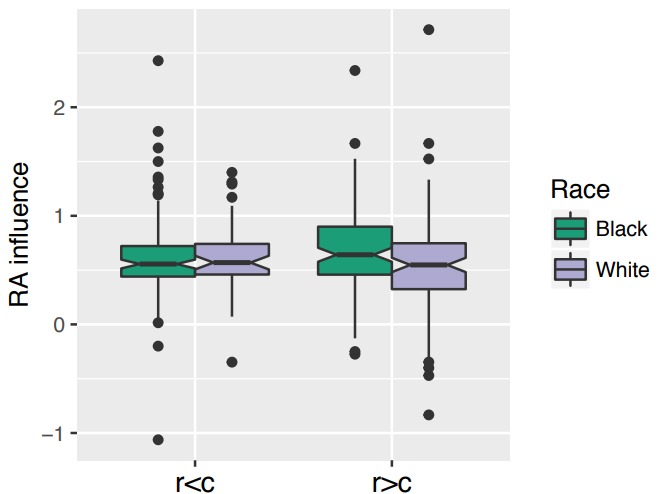
\includegraphics[width=0.5\textwidth]{Figures/influence_of_risk_score.png}
	\caption{Influence of the risk score on defendants whose risk assessment was lower than the average control group prediction ($r<c$) and for defendants the risk assessment was higher than the average control group prediction ($r>c$).}
    \label{fig:influence risk score}
\end{figure}

\subsection{Limitations and Discussion}
The study of \citet{green2019disparate} showed that algorithmic risk assessment can reinforce unfairness in human decision making. Although the performance increased under the influence of the risk assessment tool, participants were not able to beat the risk assessment. Furthermore, participants were not able to judge their own or the risk assessments performance. All these findings imply that risk assessment providing numerical scores are potentially having unforeseen side effects. Hence, it is absolutely necessary to understand the influence and interactions between human and algorithmic decision making, in order to design efficient assessment tools. 
Finally this study was conducted on Amazon Mechanical Turk and there were no real judges involved. Also participants saw the defendants profile but had no face to face conversation, as it would happen in a courtroom. It is therefore for future work to investigate the influence of risk assessment in actual court rooms. 

\section{Predict Responsibly}
\label{sec:paper2}
One way of modelling the human-machine interactions considers the cases where the human is not always the final decision maker so the machines and humans can decide jointly. A machine learning model first evaluates a sample, then either makes a decision by itself or proceeds to pass it on to the external human decision maker. Aim of this approach is for machine learning model to learn the weaknesses and strengths of the human decision makers so that it can adapt to them to better serve the systems objectives.
\par In this chapter we will first introduce the concept of having a pass option. Then we will discuss the motivations and the formulations of the \citet{madras2018predict} paper, their experimental setup and lastly the results they reported.

\subsection{PASS option}
Learning to defer first needs a formulation of having a pass option, which can simply be made through a gating variable deciding who to predict. Final prediction is made as follows:
\begin{equation}
    \hat{Y} = (1-s)\hat{Y}_{M} + s\hat{Y}_{D}
\end{equation}
where $\hat{Y}_{M}$ is the prediction of the machine learning model, $\hat{Y}_{D}$ is that of the external decision maker and $s$ is the so-called gating variable which is 1 for rejections and 0 otherwise.

One of the influential papers to tackle this flexible binary classification problem is explored by  \citet{bartlett2008classification}, where the rejection incurs a pre-specified constant loss. Authors suggest the minimization of a surrogate convex loss function that is analogous to hinge loss used in support vector machines (SVMs). Their objective function uses a gating variable as\footnote{Notation has been adapted to labels denoted by $\{0,1\}$, instead of $\{-1,1\}$ of the paper}
\begin{equation}
s = 
\begin{cases} 
  1 & \text{if} |\hat{Y}_{M}| \leq \frac{1}{2} + \delta \\
  0 & \text{otherwise} 
\end{cases}
\end{equation}
which may be viewed as defining a band around the decision boundary where the model is not confident about the prediction.

\citet{cortes2016learning} build upon this idea and formalize the concept of rejection learning. They find the earlier confidence based rejection inadequate as the method fails to find the optimal rejection region if such region cannot be defined as a function of the best decision boundary. Instead, they suggest a more general approach by defining the objective function as
\begin{equation}\label{eq:pr-loss_reject}
    \mathcal{L}_{reject}(Y,\hat{Y}_M, \hat{Y}_D, s) = \sum\limits_i [(1-s_i) \ell(Y_i, \hat{Y}_{M,i}) + s_i \gamma_{reject}]
\end{equation}
\par Since its minimization is computationally hard, authors provide two surrogate loss functions while providing the theoretical guarantees for convergence as well.

\citet{madras2018predict} propose learning to defer, as a natural extension of rejection learning. Instead of assigning a constant penalty to rejected samples, their model also considers the impact of the external decision maker and assigns a per-sample loss accordingly. The objective function they use is a modification of the \eqref{eq:pr-loss_reject}:
\begin{equation}\label{eq:pr-loss_defer}
    \mathcal{L}_{defer}(Y,\hat{Y}_M, \hat{Y}_D, s) =  \sum\limits_i [(1-s_i) \ell(Y_i, \hat{Y}_{M,i}) + s_i \ell(Y_i, \hat{Y}_{D,i}) + s_i \gamma_{defer}]
\end{equation}
\par When machine predicts, both functions assign the same loss value. However, when the decision is passed to the decision maker, we now account for the loss resulting from the decision maker's predictions as well. It is easy to see that for a decision maker (DM) that outputs constant loss, the two objectives are equivalent. Authors also experimentally show that the learning to defer objective is a generalization of the rejection learning one in the fairness case as well.

\subsection{Learning to defer}
The authors motivate their approach by saying the model should predict only if its predictions are reliably aligned with the system’s objectives, which often include accuracy and fairness. They deem the rejection learning approach as inherently non-adaptive as it fails to generalize to real-world scenarios by assigning a constant cost to each rejection. Madras et al. exemplify cases where the DM is less accurate than the machine learning model (either overall, or on subsets of data) or biased against certain subgroups. In such cases, assigning the same cost to each rejection might not align with the system objectives. We may prefer to pass the decision to DM only where DM is reliable and fair. Thus, they state the main contribution of their paper is the formulation of adaptive rejection learning as learning to defer (as well as it being the first paper to consider the fairness impact of the rejection process).

In short, paper's primary inspiration is provided in the name of the paper, if we want to \textit{predict responsibly} we should not consider the model in isolation but also take its impact into account. Even for a state-of-the-art model, its true impact comes as a result of its interaction with the external processes. Therefore, the authors attempt to train the model not by itself, but rather as a part of a larger pipeline which includes the external processes.

The authors provide two formulations to optimize the learning to defer objective \eqref{eq:pr-loss_defer}. For both, they interpret the system as a mixture between model and DM predictions, with the probability of deferal $\pi$ being the mixing coefficient such that $s \sim Ber(\pi)$. Noting the $\pi$ and $\hat{Y}_M$ are the functions of the input $X$ parametrized by $\theta$, the loss function to minimize becomes
\begin{equation}\label{eq:pr-loss_defer_expectation}
\begin{split}
   \mathcal{L}_{defer}(Y,\hat{Y}_M, \hat{Y}_D, \pi; \theta)  
   & = \mathbb{E}_{s \sim Ber(\pi)} \mathcal{L}(Y,\hat{Y}_M, \hat{Y}_D, s; \theta) \\
   & = \sum\limits_i \mathbb{E}_{s \sim Ber(\pi)} [(1-s_i) \ell(Y_i, \hat{Y}_{M,i}; \theta) + s_i \ell(Y_i, \hat{Y}_{D,i})]
\end{split}
\end{equation}
\par First formulation uses post-hoc thresholding, similar to aforementioned confidence based rejection approach. It assumes the mixing coefficient to be a function of $\hat{Y}_M$ alone and to be either 1 or 0 ($\pi \in \{ 0,1 \}$). These assumptions make the calculations over expectations in \eqref{eq:pr-loss_defer_expectation} trivial. Another advantage of this method is that  the thresholds can be trained post-hoc on an existing binary classification model.

Second formulation uses continuous $\hat{Y}_M$ and $\pi \in [0,1]$ to learn smooth thresholds, end-to-end on top of a predictor. Neural networks could be used to parametrize the model, which in turn can be optimized directly by gradient descent. Paper uses concrete relazation method \citep{jang2016categorical}, \citep{maddison2016concrete} to sample gradients through expectation. They allow $\pi$ to be a function of both model predictions $\hat{Y}_M$ and the input $X$, as DM's expected loss may change differently than the model's, as a function of $X$. They additionally stop the gradient from $\pi$ from backpropagating through $\hat{Y}_M$ to not make it dependant on $\pi$.

Lastly, they choose equalized odds \citep{hardt2016equality} as their fairness metric. Equalized odds require false positive and false negative rates to be equal between two sensitive groups. They regularize the loss above \eqref{eq:pr-loss_defer_expectation} to obtain fair classification as follows:
\begin{equation}
    \mathcal{L}_{defer}(Y,\hat{Y}_M, \hat{Y}_D, \pi; \theta) = \mathbb{E}_{s \sim Ber(\pi)} \mathcal{L}(Y,\hat{Y}_M, \hat{Y}_D, s; \theta) + \alpha_{fair} \mathcal{R}(Y, \hat{Y}_M, \hat{Y}_D, s)
\end{equation}
The regularization term is a continuous relaxation of disparate impact (DI) as
\begin{equation}
    \mathcal{R}(Y, \hat{Y}_M, \hat{Y}_D, s) = \frac{1}{2} (DI_{Y=0}(Y,A,\hat{Y}) + DI_{Y=1}(Y,A,\hat{Y}))
\end{equation}
where
\small{
\begin{equation}
    DI_{Y=i}(Y,A,\hat{Y}) = | \mathbb{E}_{\hat{Y}\sim Ber(p)} (\hat{Y}=1-Y|A=0,Y=i) - \mathbb{E}_{\hat{Y}\sim Ber(p)} (\hat{Y}=1-Y|A=1,Y=i) |
\end{equation}
}

\subsection{Experimental setup}
Paper use two datasets: Heritage Health Prize (https://www.kaggle.com/c/hhp) and COMPAS \citep{larson2016we}. In COMPAS, they try to predict defendant's recidivism (committing a crime on bail) without discriminating by race. In Heritage Health the concern is predicting the Charlson Comorbidity Index (CCI), without discriminating by age. The authors binarize the CCI as zero/greater than zero to transform it into a binary classification problem.

\begin{table}[ht]
    \centering
    \begin{tabular}{|c|c|c|}
    \hline 
     & COMPAS & Heritage Health \\ 
    \hline 
    Label to predict & Recidivism & Charlson Index (0 or not) \\ 
    \hline 
    Sensitive attribute & Race (black vs non-black) & Age (under vs over 70 years old) \\ 
    \hline 
    Withheld information & Violent recidivism & Primary condition group \\ 
    \hline 
    Inconsistency subgroup & People below the mean age & Males \\ 
    \hline 
    \end{tabular}
    \caption{Details of the datasets}
    \label{tab:pr-datasets}
\end{table}

Authors consider three different scenarios to evaluate their model:
\begin{enumerate}[A)]
    \item High-accuracy DM: ignores fairness
    \item Highly-biased DM: strongly unfair
    \item Inconsistent DM: ignores fairness (noisy)
\end{enumerate}
\par As obtaining real-life decision data is difficult, they use ``semi-synthetic'' data: they simulate DM's on real data. In each scenario DM receives extra information in training. For COMPAS, this is the defendant’s violent recidivism; for Health, this is the patient’s primary condition group. For highly-biased DM, they train decision makers with negative regularization ($\alpha_{fair} = -0.1$) to encourage high disparate impact. For inconsistent DM, they first choose a subset, which is males in Health and people below the mean age in COMPAS. Then they flip DM’s predictions  on that subset with 30\% probability. All the details regarding the datasets can be see in Table \ref{tab:pr-datasets}. This paper will only illustrate the results from the COMPAS dataset because of the space reasons, although both results demonstrate similar trends.

\subsection{Results and discussion}
The authors found the post-hoc and end-to-end models performed similarly for scenarios A and B, so they presented results only for the post-hoc formulation, as it is simpler. However, post-hoc model cannot adapt to the inconsistent DM scenario as the deferral probability has to be a function of input $X$ as well, so presented results for scenario C is from the end-to-end model.

\begin{figure}[ht]
\centering
\begin{subfigure}[t]{0.5\textwidth}
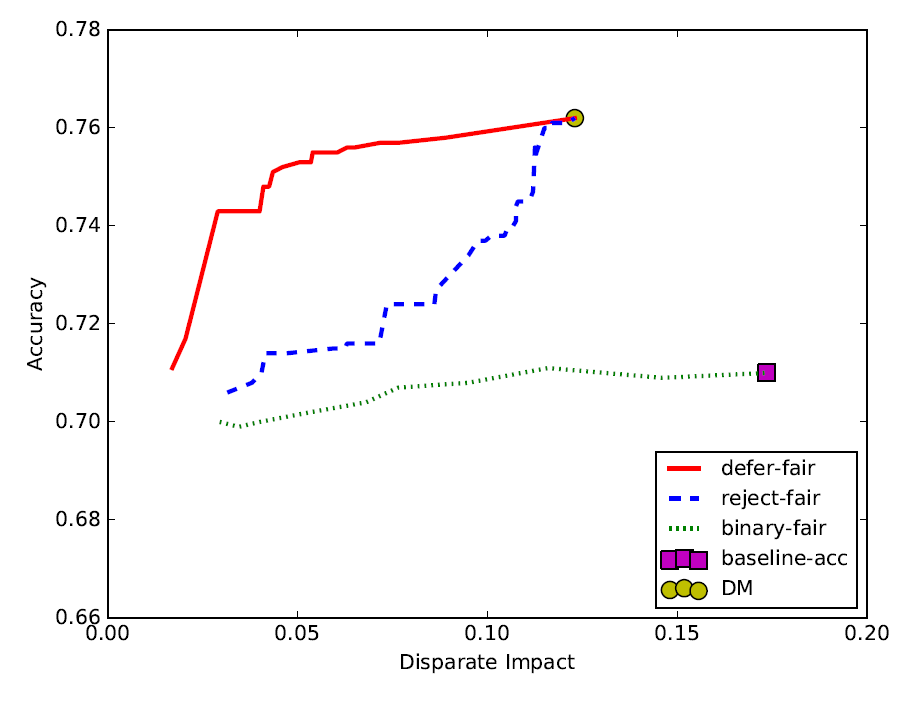
\includegraphics[width=\textwidth]{Figures/compasHighAcc.PNG}
\caption{COMPAS, High-accuracy DM}
\label{fig:pr-resHighAcc}
\end{subfigure}%
\begin{subfigure}[t]{0.5\textwidth}
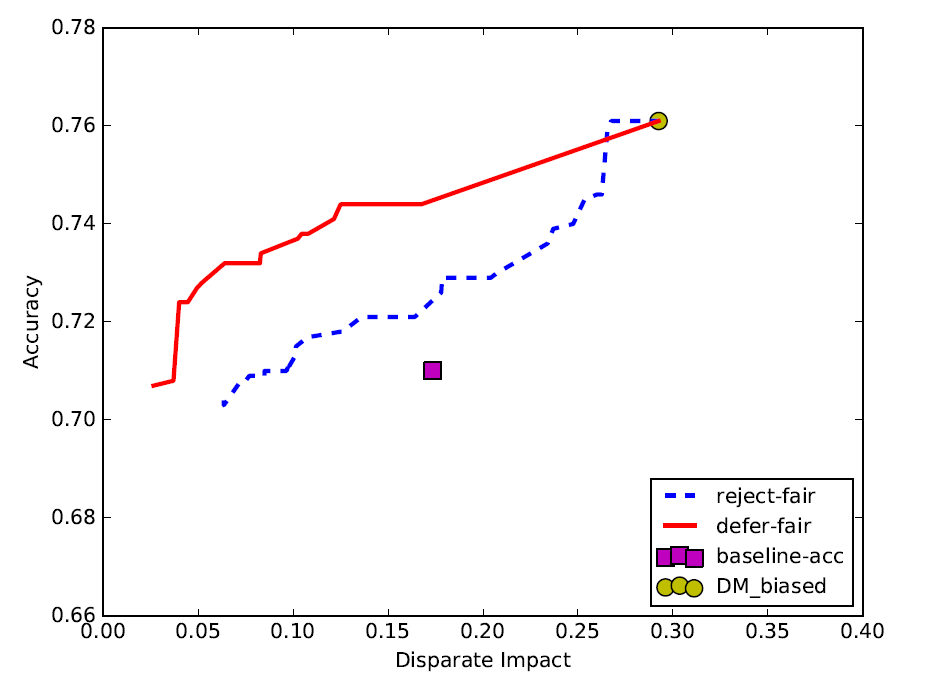
\includegraphics[width=\textwidth]{Figures/compasHighlyBiased.PNG}
\caption{COMPAS, Highly-biased DM}
\label{fig:pr-resHighBias}
\end{subfigure}
\caption{Results for scenarios A and B on COMPAS dataset}
\label{fig:pr-resAB}
\end{figure}

Figure \ref{fig:pr-resHighAcc} shows that learning to defer achieves a better accuracy-fairness trade-off than rejection learning. It is also worth noting that both models outperform the binary baselines by incorporating the predictions of the DM, which has access to extra information that the model does not have (cf. Table \ref{tab:pr-datasets}).

Figure \ref{fig:pr-resHighBias} shows that the learning to defer is advantageous over rejection learning in the highly-biased DM setting as well. Unlike rejection learning, deferral rates over the different values of the sensitive attributes (not shown here) differ for learning to defer model. This, together with the aforementioned results, hint at learning to defer model adapting to the biases of the DM and deferring decisions accordingly.

\begin{figure}[ht]
\centering
\begin{subfigure}[t]{0.4\textwidth}
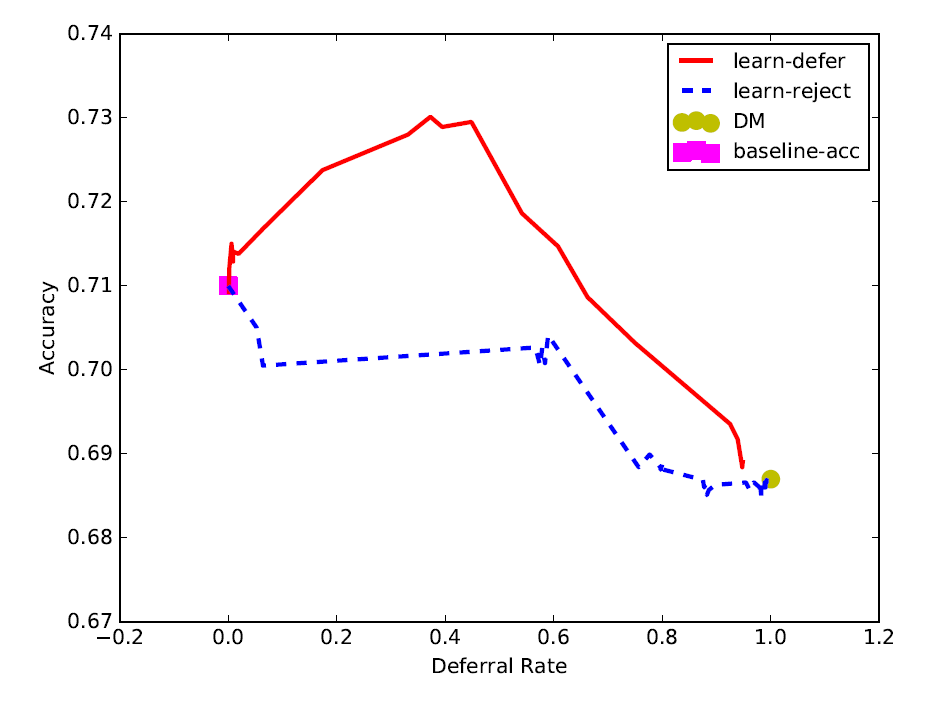
\includegraphics[width=\textwidth]{Figures/compasInconsistent.PNG}
\caption{COMPAS, Inconsistent DM}
\label{fig:pr-resIncons}
\end{subfigure}%
\begin{subfigure}[t]{0.6\textwidth}
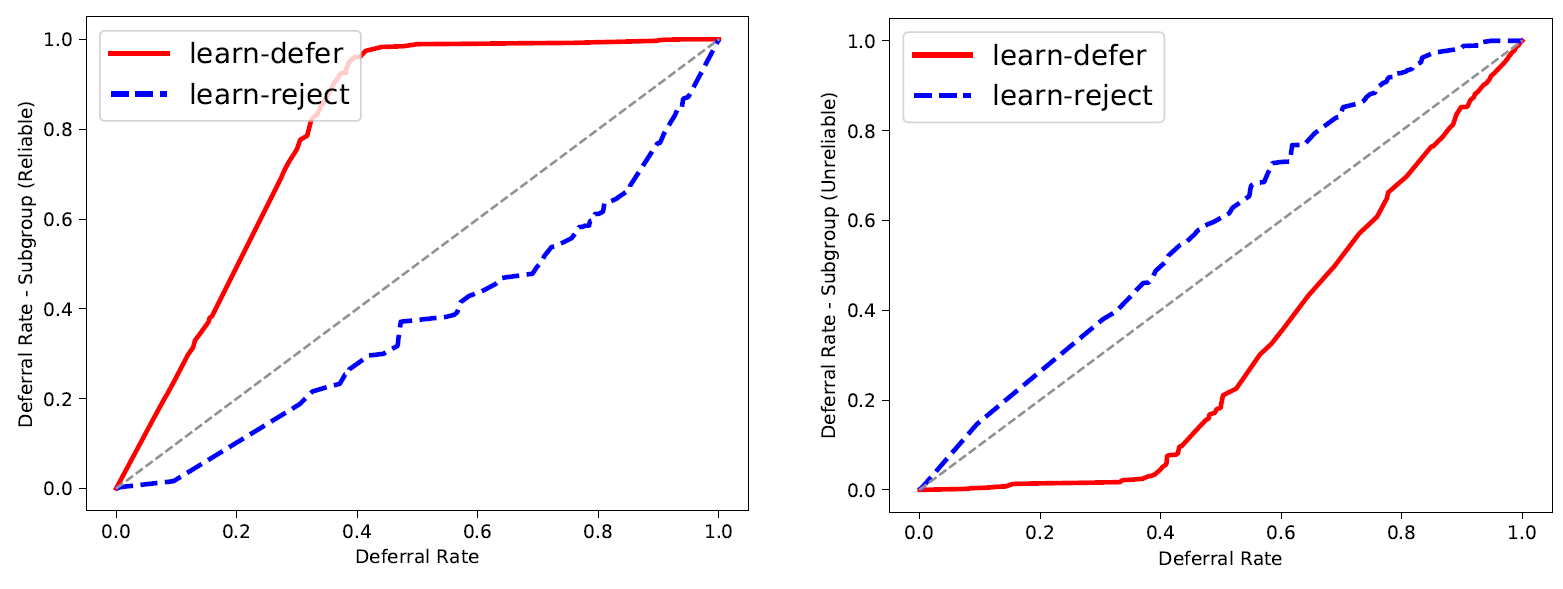
\includegraphics[width=\textwidth]{Figures/compasDeferralRatesC.PNG}
\caption{COMPAS, Inconsistent DM Deferral Rates}
\label{fig:pr-resDeferC}
\end{subfigure}
\caption{Results for scenario C on COMPAS dataset}
\label{fig:pr-resC}
\end{figure}

We lastly look at the inconsistent DM scenario, whose reliability differs across different subgroups. We see in Figure \ref{fig:pr-resIncons} the model consistently being more accurate than the DM, but the optimal results are obtained by using a DM-model mixture rather than replacing the model completely. This is the very premise of the inconsistent DM scenario and such a result is arguably only achievable by an adaptive rejection scheme. Figure \ref{fig:pr-resDeferC} allows a closer look at what goes under the hood. In line with the expectations, model prefers to defer more on DM's reliable subgroup and predicts by itself where DM is unreliable. Curious reader should note that the original paper provides a more detailed discussion on the various trends over all the results.

In short, we can say the concept of deferral (or adaptive rejection) can be a powerful framework, illustrated by the results in this section. Such a framework can be applied to many complex domains where humans and machines work together. Criminal justice and medical diagnosis are only two examples. This idea could also be seen as a necessity because the role of machine learning grows more as it becomes heavily integrated in many real-world problems alongside humans.

\section{Improving fairness and accuracy through matching}
\label{sec:paper3}

One approach which can increase fairness and accuracy of decisions is to optimize the matching between decision makers(DM's) and decisions. This way bias or lack of predictive ability of DM's can be mitigated, while still using human DM's for the final decisions. The paper Enhancing the Accuracy and Fairness of Human Decision Making \citep{2018arXiv180510318V} shows how such a matching problem can be approached. In this chapter we show how the problem was formulated, what algorithms to solve the problem were proposed, and review the main results and limitations of the paper.
  
\subsection{Problem Formulation}
The paper defines the matching problem as follows. There are T time-steps, and at each time-step there are m binary decisions to be taken. Given a number of DM's greater than m, find an assignment of DM's to decisions at each time-step, such that over time we optimize the utility and fairness of those decisions.

Each decision has a binary outcome and is denoted using $d_j(X_i,S_i)$.
Where $X_i \in \mathbb{R}^d$ are non-sensitive features,  $S_i \in \{0,1\}$ stands for a binary sensitive feature. $d_j(X_i,S_i)$ means the decision of the $j^{\text{th}}$ DM assigned to the $i^{\text{th}}$ decision.

In the paper it is assumed that every DM knows the true conditional probability $P(Y_i|X_i,S_i)$. Where $Y_i \in \{0,1\}$ stands for the ground truth decision.
But each DM has her own thresholds $\theta_{j,s}$, and only if the conditional probability is greater equal her own threshold, then the DM will decide with 1.
These thresholds can be different for a DM, for the two different sensitive attributes, ergo $\theta_{j,S_1}\ne \theta_{j,S_2}$, which allows modelling biases. For a DM j and a decision $(X_i,S_i)$ we get the following decision function.
$$
d_j(X_i,S_i) = 
\begin{cases}
1, & {\text{if } P(Y_i=1|X_i,S_i)\ge \theta_{j,S_i}} \\
0, & \text{otherwise}
\end{cases}
$$
\\
The utility of a decision is defined as a benefit of 1 if both ground-truth and decision are 1, minus a cost of c if the decision is 1. So only \emph{True Positive} and \emph{False Positive} are used as part of the utility definition.
$$u(d,c)=\mathbb{E}[Yd(X,S)-cd(X,S)]=\mathbb{E}[d(X,S)(P_{Y|X,S}-c)]$$
To measure the utility of the proposed sequential human decision problem, the utility function is generalized. Let $v_i(t)$ be the assigned DM to decision i in round t, then the utility function can be rewritten as the mean utility over all time-steps and decisions per time-step.

$$u_{\le T}(d_{v_i(t),i,t},c)=\frac{1}{mT}\sum_{t=1}^T \sum_{i=1}^m d_{v_i(t)}(x_i(t),s_i(t))(p_{Y=1|x_i(t),s_i(t)}-c)$$
\\
Where $(x_i(t),s_i(t))$ stands for the i-th decision at timestep t.

\subsection{Proposed Algorithms}
\textbf{Known Thresholds:} First it's assumed the thresholds of all DM's are known. 
\\\\
If no fairness constraint is required, the optimal assignment problem can be reduced to a maximum weighted bipartite matching problem.
For this create a bipartite graph with DM's on one side, and decisions on the other. By assigning weights to the connecting edges in the following way, maximum weighted matching provides us with the optimal assignment in quadratic time.
$$
w_{ji} = 
\begin{cases}
P(Y_i=1|X_i,S_i)-c, & \text{if } P(Y_i=1|X_i,S_i)\ge \theta_{j,S_i} \\
0, & \text{otherwise} \\
\end{cases}
$$ 

To enforce a fairness constraint, more specifically disparate impact, a different algorithm has to be used. Let $b_{S_i}$ be the expected benefit given sensitive feature $S_i$. Disparate impact is defined as follows.
$$DI=|b_{s=1}-b_{s=0}|\le \alpha$$
Now let $b^*_{S_i=s}$ be the expected benefit if we choose the optimal decision, while satisfying the disparate impact constraint. We can attempt to enforce disparate impact by extending the utility function with the following inequalities for each sensitive feature value.
$$ m_{S=s}(b_{S=s}^*-\alpha)\le \sum_{\forall (i,j), S=s}\mathbbm{1} (w_{ji}= 0)$$
$$\sum_{\forall (i,j), S=s}\mathbbm{1} (w_{ji}= 0) \le  m_{S=s}(b_{S=s}^*+\alpha)$$

Which limits the expected benefit of that sensitive feature value to a bound of $\alpha$ around the optimal benefit $b^*_{S_i=s}$.
Note that the second inequality can be rewritten as
$$\sum_{\forall (i,j), S=s}\mathbbm{1} (w_{ji}\ne 0) \ge m_{S=s}(b_{S=s}^*+\alpha)$$

This allows us to reduce the optimal matching problem at each time-step to a bounded color matching problem which can be solved using a bi-criteria algorithm with $\frac{1}{2}$-approximation guarantee in polynomial time \citep{MastrolilliS13}.
\\
\\
\textbf{Unknown Thresholds: } In case the DM's thresholds are unknown, they propose in the paper to first assume prior beta-distributions of the thresholds. Then, using information learned per time-step, we can update the posterior distribution of each DM for each sensitive attribute value $S=s$.
$$\theta_s\sim \text{Beta}(\alpha,\beta)$$
Given the true conditional probability $P(Y=1|X,S)$, and a number of time-steps where a DM was chosen to decide, allows the distribution to be updated. We can check which is the highest conditional probability $P(Y=1|X,S)$ where the DM decided $d(X,S)=0$, and which is the lowest conditional probability $P(Y=1|X,S)$ where the DM decided $d(X,S)=1$.
$$max(0,\theta^L_s)\le \theta_s \le min(1,\theta^H_s )$$
This allows us to update the posterior beta distribution of a DM using the following formula.

$$P(\theta_s | D)=\frac{\Gamma(\alpha+\beta)(\theta^H_s-\theta_s)^{\alpha-1}(\theta_s-\theta^L_s)^{\beta-1}}{\Gamma(\alpha)\Gamma(\beta)(\theta^H_s-\theta^L_s)^{\alpha+\beta-1}}$$ 

Where $\Gamma(x)$ is the Gamma-function. At the beginning of the next round the new threshold can then be sampled from this conditional distribution. $$\theta_s(t+1)\sim P(\theta_s(t)|D(t))$$

\textbf{Regret:}
Regret is defined as the difference in utility between the chosen assignment $u_{\le t}(d,c))$ and optimal assignment $u_{\le t }^*(d,c)$.
$$R(T)=u_{\le T}(d,c))-u_{\le T }^*(d,c)$$
When sampling from the conditional distribution, the expected regret will shrink in $O(\sqrt{T})$.
Additionally they can show that if $\theta_s$ is chosen as the $argmax(P(\theta_s(t)|D(t)))$, then the expected regret will only change linearly in $\Theta(T)$. This is because choosing the maximum a posteriori as the next threshold leads to insufficient exploration.  

\subsection{Experiments \& Results}

The results presented here are based on the COMPAS recidivism prediction dataset \citep{larson2016we}. Additionally the paper provides the results of the experiments on a self-made synthetic dataset, with similar outcome.

For this experiment they used 20 decisions per time-step, and 197 time-steps. Because the COMPAS dataset doesn't contain information on DM's, they generated the DM's by sampling decision thresholds from beta-distributions. In total there were 60 DM's with varying decision boundaries which could be assigned at each time-step to decisions. In order to calculate a conditional probability $P(Y|X,S)$ they used 25\% of the data to train a logistic regression classifier. The experiments were conducted on the other 75\% of the data.
\\\\
Four types of results are compared:\\
\textbf{Random}: Random assignment between DM's and decisions\\
\textbf{Optimal}: Choosing the optimal decision threshold per decision, given true posterior probability and disparate impact. (Note: no DM's involved)\\
\textbf{Known $\theta$}: assumes the thresholds of the DM's are known, and we use the proposed algorithms to assign matchings at each time-step.\\
\textbf{Unknown $\theta$}: assumes the thresholds of the DM's are unknown, and we use the proposed algorithms to assign matchings at each time-step.\\

\begin{figure}[ht]
    \centering
    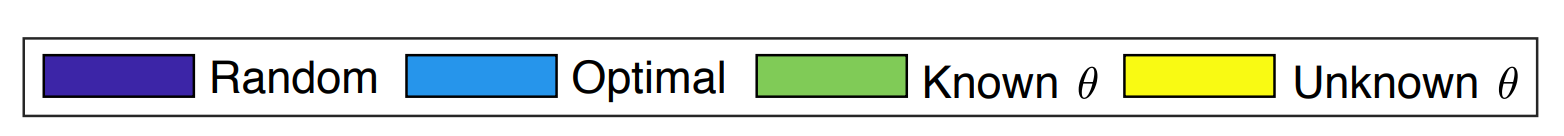
\includegraphics[width=0.7\textwidth]{Figures/matching_results_part2.png}
\end{figure}
\begin{figure}[ht]
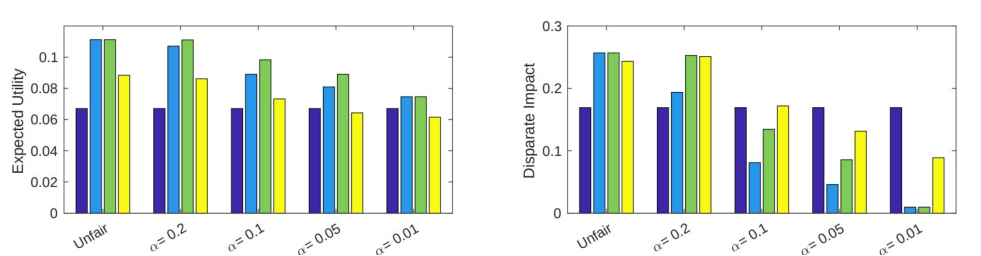
\includegraphics[width=\textwidth]{Figures/matching_results_part1.pdf}
\label{fig:ma-results}
\caption{For expected utility, the higher the better, for disparate impact, the lower the better. $\alpha$ stands for the allowed disparate impact difference. }
\end{figure}
As the results indicate, this new assignment of DM's to decisions increases overall utility, in comparison to a random assignment, for both known and unknown thresholds. If required, it can also reduce disparate impact. If the thresholds of the DM's are known, then the results optimal decision rule can be approximated.
Note that the utility can only be higher than the optimal solution, if the disparate impact value is also higher. 

A notable difference to the optimal assignment is in case of a disparate impact limit. Because at each time-step the algorithms can only match a limited amount of DM's and problems, it's not guaranteed that an assignment can be found, which is within the allowed disparate impact difference.
\\\\
They stated in the paper two additional benefits. They could show that high diversity between DM's helps to ensure fairness. Additionally their algorithms can ensure fairness even if a high percentage of DM's (i.e. 50\%) are biased.

\subsection{Limitations, Critique \& Future Work}

There are several limitations which should be addressed in future work.
\begin{itemize}
  \item It assumes the conditional probability $P(Y|X,S)$ is known to all DM's. Ergo it's assumed all DM's have the same predictive ability. 
  \item The problem is setup as a 1-human 1-problem matching at each time-step with many iterations. This choice allows a reduction of the optimal matching to graph-type problems. But different problem definitions might allow more flexible solutions, especially in regard to alternative fairness constraints.
  \item The proposed algorithms can attempt to enforce fairness constraint only at each time-step independently, and only through varying matching of DM's to decisions. As seen in the results, in many cases, this leads to fairness constraints not being enforced to the specified value.
  \item The decisions of the DM's are static over time. DM's don't learn anything from past decisions in the current setup. \item There are no datasets available, where the decision per DM are known, which forces the use of synthetic DM's. 

\end{itemize}
\textbf{Limitations with respect to other fairness notions}
\begin{itemize}
\item While disparate impact, equality of opportunity, and disparate mistreatment to a certain extent can be enforced by the proposed algorithm, more complicated fairness notions won't be able to be reduced to a bounded color matching problem. For such cases a different algorithm is required. 
\item Additionally, in terms of individual fairness constraints, the proposed algorithm seems to be vulnerable. As an example, the decision for an individual is dependent on the selection of other decisions at that specific time-step. The algorithm then might choose a very biased DM with respect to the individuals sensitive attribute, just to attempt to hold for the disparate impact condition
\end{itemize}

\section{Discussion and Conclusion}
\label{sec:conclusion}
In this paper we studied three different patterns on how to combine human and machine decision makers. The first pattern, algorithmic risk prediction, supports human decisions by providing an additional risk score. While this helps to increase the performance, we saw that it could have unforeseen negative effects on the fairness of the decision process. In the second pattern, learning to defer, machines take a more active role and are allowed to make decisions on their own in certain cases. This pattern is able to increase fairness, but at the cost of a clear responsibility and humans having the upper hand in the decision process. In the third pattern, the algorithm took the most passive role as it assigned humans to decision problems, but did not make a decision nor support the human in making the decision.

Humans and machines both have their relative merits and we believe the greatest potential lies in their cooperation. Nonetheless, attention must be paid to how this cooperation is to be established. We have claimed in the preceding sections that there is not a gold standard on how to combine human and machine decisions and there is much work to be done. The way to a better cooperation and utilization is paved with many nuances and pitfalls. Such nuances and pitfalls may seem to differ in scale, but we should not disregard any aspect in this process by deeming it as insignificant, as we could be still unaware of the complex details of human-machine interaction. We believe transparency, explainability and accountability become especially important and we should pay an increasing attention to how we should establish cooperation, as humans and machines assist each other more than ever.


\section*{Division of Labour}

Workload has been divided as follows: 
\begin{itemize}
    \item Everyone read each paper,
    \item Each paper was discussed in the group of three over three meetings,
    \item We divided the workload by assigning one paper to one student, 
    \item Everyone wrote the section of this paper describing their paper,
    \item Everyone made the slides describing their paper,
    \item General slides and general chapters of the paper were done together,
    \item Everyone had a look at all sections/slides to make them look coherent.
\end{itemize}

%\pagebreak
\bibliography{Bibliography}
\bibliographystyle{apalike}


\end{document}
